\documentclass[tikz,border=2pt]{standalone}
\usepackage{tikz}
\begin{document}
  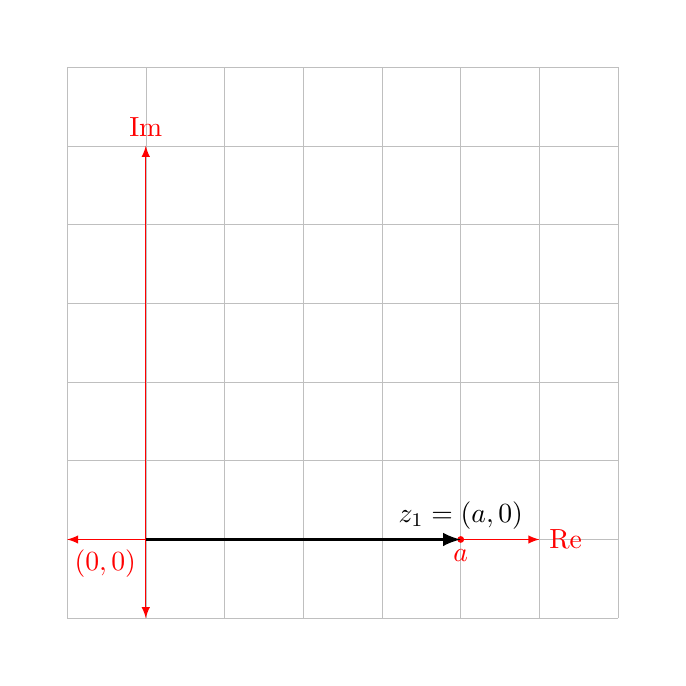
\begin{tikzpicture}
    \fill[white] (-1.5,-1.5) rectangle (6.5,6.5);
    \draw[lightgray,very thin] (-1,-1) grid (6,6);
    \draw (0,0) node[red,below left]{$(0,0)$};
    \draw[red,latex-latex] (-1,0) -- (5,0) node[right]{Re};
    \draw[red,latex-latex] (0,-1) -- (0,5) node[above]{Im};
    \draw (4,0) node[red,below]{$a$};
    \draw (4,0) node[above]{$z_1=(a,0)$};
    \filldraw[red] (4,0) circle(1pt);
    \draw[very thick,-latex] (0,0) -- (4,0);
  \end{tikzpicture}
\end{document}
\end{document}
